
	\subsubsection{Use-Case Instance - uciugSecurelyUseSystemFailLogin:ugSecurelyUseSystem}
	
	use case instance for the user goal use case \msrcode{ugSecurelyUseSystem} illustrating a simple interaction scenario primarily handled by an administrator in a concrete situation.
	In this instance a captcha test is asked after 3 failed attempts of login. Once the \msrcode{actAuthenticated} successfully entered the right captcha, he's able to connect. 
	\begin{operationmodel}
	\addheading{usergoal Use-Case Instance}
	\adddoublerow{Instantiated Use Case}{ugSecurelyUseSystem}
	\adddoublerow{Instance ID}{uciugSecurelyUseSystemFailLogin}
	
	\addrowheading{Remarks}
	\addalphanumberedsinglerow{}{A captcha test is asked after three failed attempts of login.}
	\addalphanumberedsinglerow{}{A password reset is always possible. A mail has to be given to the system.}
	\end{operationmodel} 

	
	Figure \ref{fig:lu.uni.lassy.excalibur.examples.icrash-RE-UC-uci-uciugSecurelyUseSystemFailLogin}
	view
	
	\begin{figure}[htbp]
	\begin{center}
	
	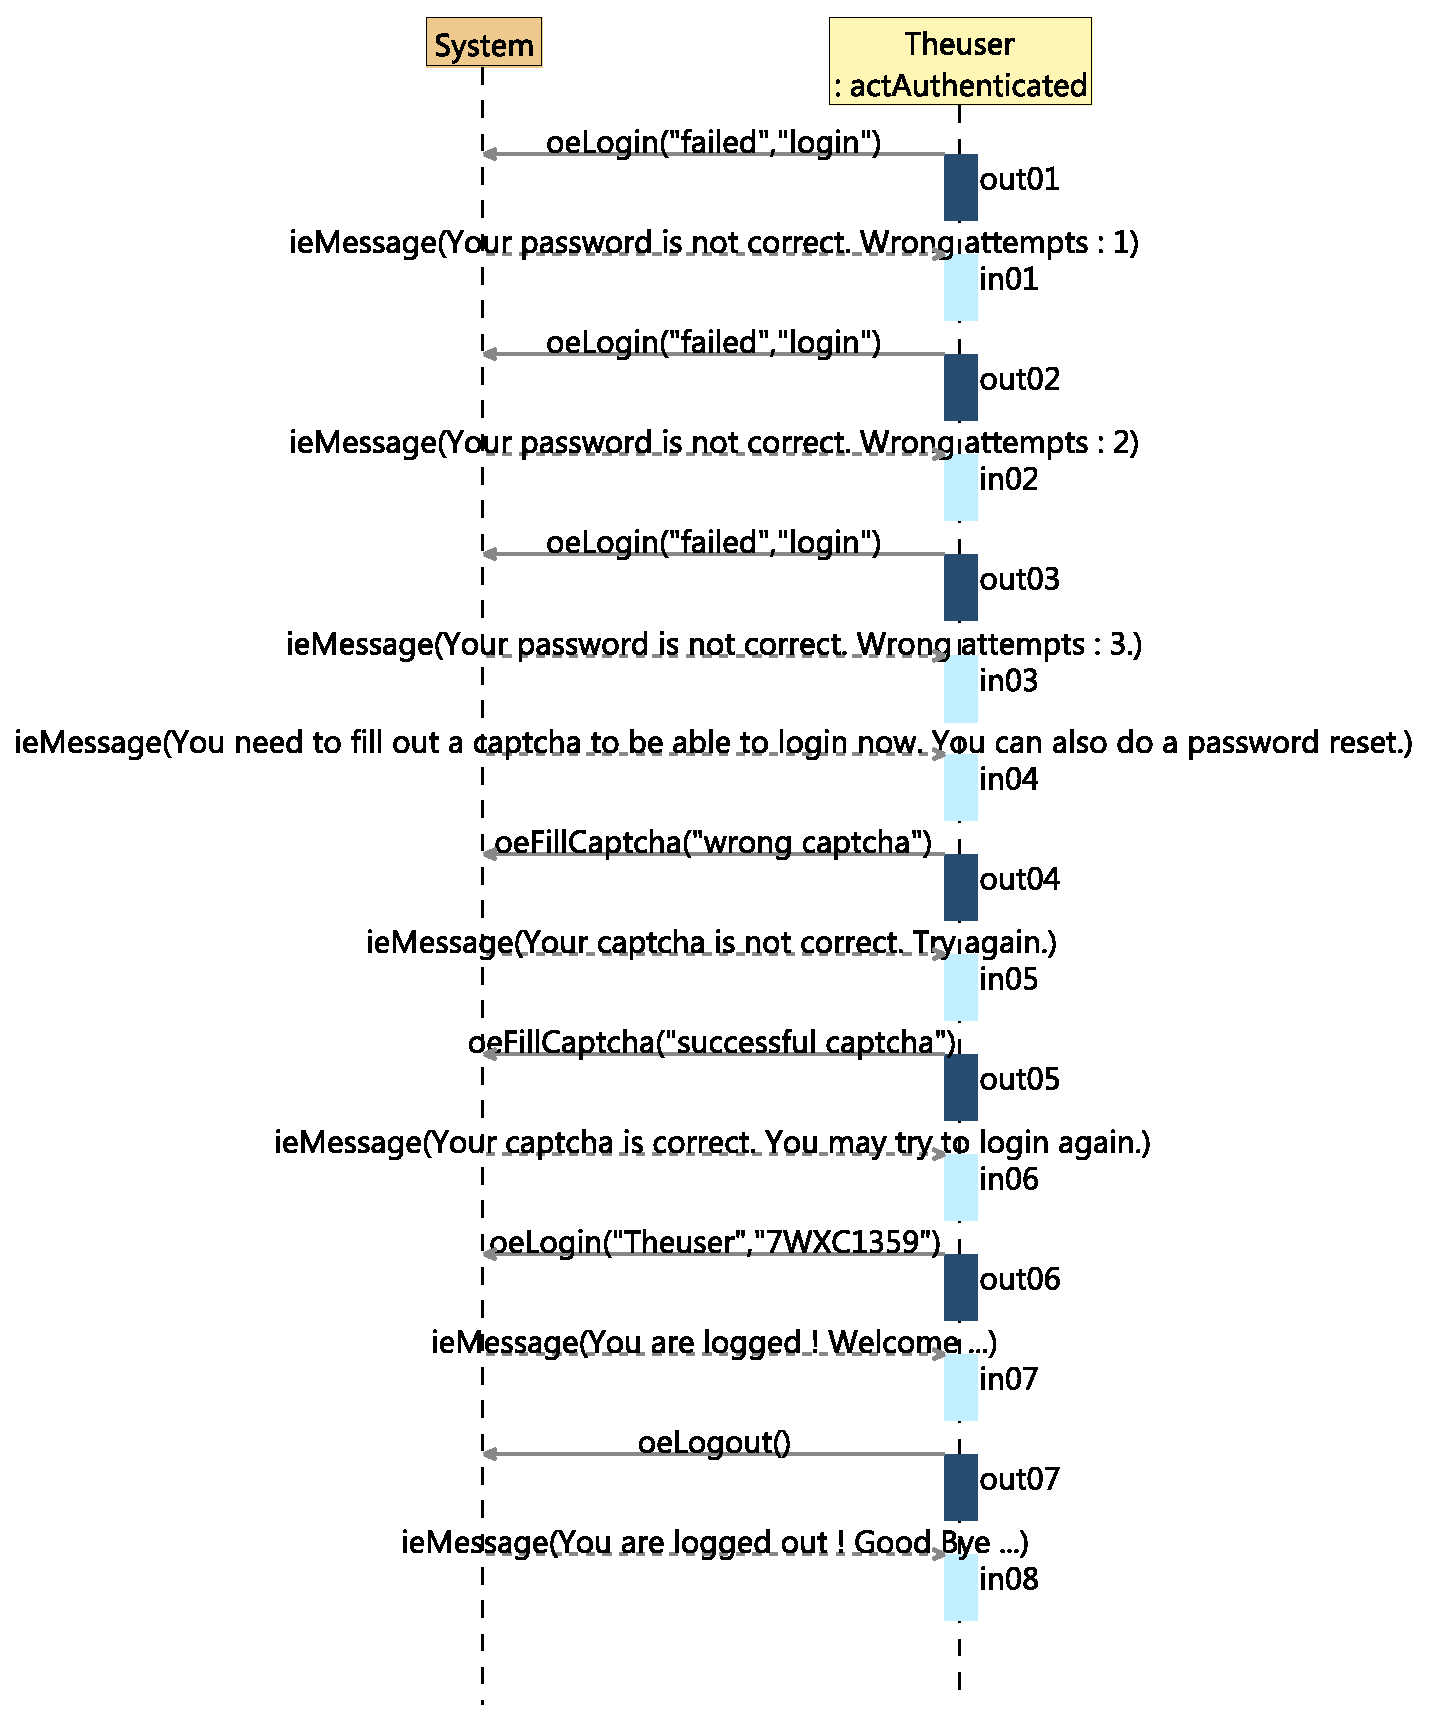
\includegraphics[
	angle=0
	]{./images-report-gen/usecase-model/usergoal/uci-uciugSecurelyUseSystemFailLogin.eps}
	\end{center}
	\caption[lu.uni.lassy.excalibur.examples.icrash Sequence Diagram: uci-uciugSecurelyUseSystemFailLogin]{}
	\label{fig:lu.uni.lassy.excalibur.examples.icrash-RE-UC-uci-uciugSecurelyUseSystemFailLogin}
	\end{figure}
	\vspace{0.5cm}
